\subsection{Differentially Heated Cavity}~\label{secDHC}

The Differentially Heated Cavity (DHC) extends the NS solver to thermally driven flows by activating the energy equation (Eq.~\eqref{eqNSEnergy}) and coupling it back to the momentum equation through buoyancy~\cite{CTTC2022Part5}. The geometry is the same square cavity as in Section~\ref{secLDC}, but with all walls stationary (no-slip) and thermal boundary conditions applied: the left wall is held at a hot temperature $T_h$, the right wall at a cold temperature $T_c < T_h$, and the top and bottom walls are adiabatic ($\partial T / \partial n = 0$). Unlike the Lid-Driven Cavity, there is no mechanical forcing; the flow is driven entirely by the temperature difference $\Delta T = T_h - T_c$, which produces density variations that generate buoyancy forces. A schematic of the problem is shown in Fig.~\ref{figDHCSchematic}.

\begin{figure}[ht]
    \centering
    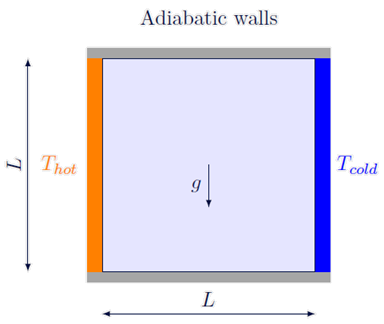
\includegraphics[width=0.45\linewidth]{Chapter3/Media/SchematicDHC.png}
    \caption{Differentially Heated Cavity schematic. The left wall is held at hot temperature $T_h$, the right wall at cold temperature $T_c$, and the top and bottom walls are adiabatic.}
    \label{figDHCSchematic}
\end{figure}

The density variation is handled through the \textbf{Boussinesq approximation}~\cite{Shames2003}, which treats the fluid as incompressible everywhere except in the buoyancy term of the momentum equation, where a linear dependence of density on temperature is assumed:

\begin{equation}\label{eqBoussinesq}
    \rho \approx \rho_0\,\bigl[1 - \beta\,(T - T_\mathrm{ref})\bigr]
\end{equation}

where $\beta$ is the thermal expansion coefficient and $T_\mathrm{ref} = (T_h + T_c)/2$ is the midpoint reference temperature. Substituting Eq.~\eqref{eqBoussinesq} into the $y$-component of Eq.~\eqref{eqNSMomentum} adds a body-force source term:

\begin{equation}\label{eqBuoyancy}
    S_y = -\rho_0\,\beta\,(T - T_\mathrm{ref})\,g
\end{equation}

This term is positive (upward) where $T > T_\mathrm{ref}$ and negative (downward) where $T < T_\mathrm{ref}$, driving the familiar convection cell: hot fluid near the left wall rises, travels along the top, descends along the cold right wall, and returns along the bottom. Equation~\eqref{eqBuoyancy} is treated as an explicit source in $b_P$ of the $y$-momentum discretization, evaluated at the current time step. The energy equation is discretized using the convection-diffusion FVM of Chapter~\ref{chapConvection}, with $\phi \equiv T$ and $\Gamma \equiv \lambda$, advanced by the same Adams-Bashforth scheme.

The flow regime is characterised by the \textbf{Rayleigh number}:

\begin{equation}\label{eqRayleigh}
    Ra = \frac{g\,\beta\,\Delta T\,H^3}{\nu\,\alpha}
\end{equation}

where $H$ is the cavity height, $\nu = \mu/\rho_0$ is the kinematic viscosity, and $\alpha = \lambda/(\rho_0 c_p)$ is the thermal diffusivity. The Rayleigh number encodes the ratio of buoyancy driving to diffusive resistance. At low $Ra$, diffusion dominates and the temperature field is nearly linear across the cavity with minimal flow velocity. As $Ra$ increases, convection intensifies, the isotherms bow progressively, and thin thermal boundary layers form on the hot and cold walls. Four cases are tested: $Ra = 10^3$, $10^4$, $10^5$, and $10^6$, at fixed Prandtl number $Pr = \nu/\alpha = 0.71$ (air). The reference solution is provided by de Vahl Davis~\cite{deVahlDavis1983}.

Validation is performed against the benchmark values of de Vahl Davis~\cite{deVahlDavis1983} using the average Nusselt number at the hot wall, defined as:

\begin{equation}\label{eqNusselt}
    \overline{Nu} = -\frac{H}{\Delta T}\,\left\langle\frac{\partial T}{\partial x}\right\rangle_{x=0}
\end{equation}

where $\langle \cdot \rangle$ denotes the wall-averaged value. The Nusselt number compares the actual heat transfer rate to the conductive rate across a stagnant fluid layer of the same thickness; it is therefore a single scalar that integrates the accuracy of both the velocity and temperature fields. Centreline profiles of $u(x = 0.5)$ and $v(y = 0.5)$ are also compared to provide a spatially resolved assessment.


\subsubsection{Model Implementation}

The DHC solver extends the Lid-Driven Cavity model with two modifications. First, the energy equation is activated and coupled to the momentum solver: at each time step, after the velocity field $\mathbf{v}^{n+1}$ is obtained from the FSM algorithm, the energy equation is advanced using the updated velocity to evaluate the convective fluxes in $R(T)$. The temperature field then provides the buoyancy source term $S_y$ (Eq.~\eqref{eqBuoyancy}) for the next time step's $y$-momentum equation. This explicit coupling is consistent with the Adams-Bashforth scheme and does not require inner iteration between the velocity and temperature equations. Second, the thermal boundary conditions are specified through the boundary configuration parameters: Dirichlet conditions for the left ($T_h$) and right ($T_c$) walls, and Neumann zero-flux conditions for the top and bottom walls.

The dimensionless parameters $\rho_0 = 1$, $c_p = 1$, and $H = 1$ are fixed throughout, with $\mu$, $\lambda$, and $\beta$ chosen to achieve the target $Ra$ and $Pr$ for each case. Initial conditions are $\mathbf{v}^0 = \mathbf{0}$ and a linear temperature profile $T^0(x) = T_h - \Delta T \cdot x / H$, which provides a smooth start and reduces the transient duration.


\subsubsection{Numerical Parameter Study}

The mesh refinement study uses the $Ra = 10^5$ base case, which presents boundary layers thin enough to be resolution-sensitive while remaining tractable at moderate mesh sizes. The average Nusselt number $\overline{Nu}$ at the hot wall is used as the scalar convergence metric, evaluated against the de Vahl Davis reference~\cite{deVahlDavis1983}. The tested mesh sizes are summarised in Table~\ref{tabDHCNumerical}.

\begin{table}[ht]
    \centering
    \begin{tabular}{|c|c|}
        \hline
        Parameter & Values \\
        \hline
        $N$ & 16,\ 32,\ 64,\ \textbf{128} \\
        \hline
    \end{tabular}
    \caption{Mesh sizes tested in the spatial refinement study for the Differentially Heated Cavity ($Ra = 10^5$, Hybrid). Bold value indicates the resolution selected for $Ra = 10^5$ and $10^6$; $N = 64$ is used for $Ra \leq 10^4$.}
    \label{tabDHCNumerical}
\end{table}

\paragraph{Mesh Refinement}
The average Nusselt number $\overline{Nu}$ at the hot wall is computed for each mesh level and compared against the de Vahl Davis reference in Fig.~\ref{figDHCRefinement}. Table~\ref{tabDHCRefine} lists the values numerically.

\begin{figure}[ht]
    \centering
    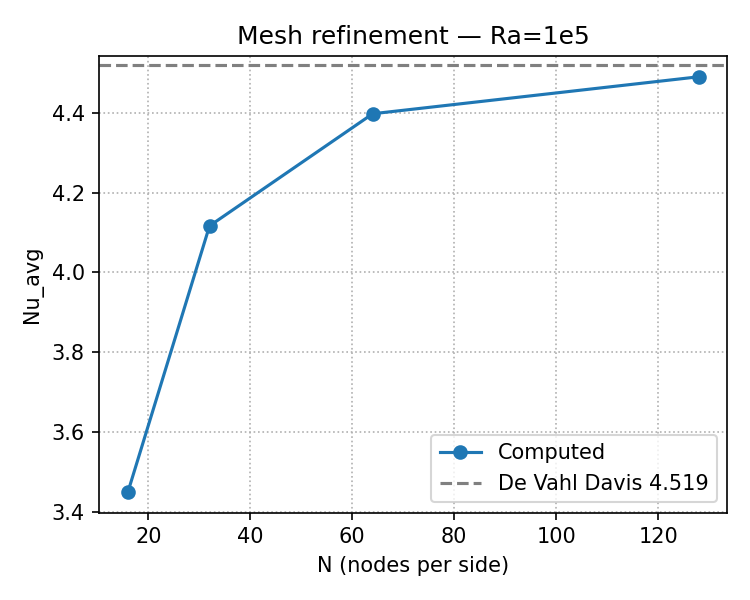
\includegraphics[width=0.55\linewidth]{Chapter3/Media/Nu_refinement.png}
    \caption{Mesh refinement study for the Differentially Heated Cavity ($Ra = 10^5$, Hybrid). Average Nusselt number $\overline{Nu}$ at the hot wall as a function of nodes per side $N$, compared against the de Vahl Davis reference~\cite{deVahlDavis1983}.}
    \label{figDHCRefinement}
\end{figure}

\begin{table}[ht]
    \centering
    \begin{tabular}{|c|c|c|}
        \hline
        $N$ & $\overline{Nu}$ & $Nu_{\max}$ \\
        \hline
        16  & 3.450 & 5.058 \\
        32  & 4.116 & 6.461 \\
        64  & 4.398 & 7.283 \\
        128 & 4.490 & 7.598 \\
        \hline
        De Vahl Davis & 4.519 & 7.717 \\
        \hline
    \end{tabular}
    \caption{Average and maximum Nusselt number at the hot wall for $Ra = 10^5$ at four mesh levels (Hybrid). Reference values from de Vahl Davis~\cite{deVahlDavis1983}.}
    \label{tabDHCRefine}
\end{table}

Richardson extrapolation over the three finest meshes yields an apparent order $p = 1.60$ and an extrapolated value $\overline{Nu}^\infty = 4.536$, which lies within $0.38\%$ of the de Vahl Davis reference. The intermediate order ($1 < p < 2$) is consistent with the Hybrid scheme: near the hot and cold walls where $Pe_k \leq 2$, the scheme applies CDS and achieves second-order accuracy in resolving the thermal boundary layers; in the convective core where $Pe_k > 2$, first-order UDS dominates. The GCI~\cite{Roache1994} at $N = 128$ is $1.27\%$, confirming adequate grid convergence. The mesh $N = 64$ is used for $Ra = 10^3$ and $10^4$; $N = 128$ is used for $Ra = 10^5$ and $10^6$ to maintain comparable boundary-layer resolution as the thermal layer thickness $\delta_T \sim Ra^{-1/4}$~\cite{Incropera2006} decreases.


\subsubsection{Model Validation}

The model is validated across all four Rayleigh number cases using the mesh resolutions established by the refinement study. The primary validation metrics are $\overline{Nu}$ and the maximum local Nusselt number $Nu_{\max}$ at the hot wall, both compared against the de Vahl Davis benchmarks~\cite{deVahlDavis1983}. The results are summarised in Table~\ref{tabDHCBenchmark}.

\begin{table}[ht]
    \centering
    \begin{tabular}{|c|c|c|c|c|c|}
        \hline
        $Ra$ & $N$ & $\overline{Nu}$ & $\overline{Nu}$ ref & Error & $Nu_{\max}$ \\
        \hline
        $10^3$ & 64  & 1.116 & 1.118 & $0.15\%$ & 1.500 \\
        $10^4$ & 64  & 2.232 & 2.243 & $0.51\%$ & 3.486 \\
        $10^5$ & 128 & 4.490 & 4.519 & $0.64\%$ & 7.598 \\
        $10^6$ & 128 & 8.562 & 8.800 & $2.71\%$ & 16.372 \\
        \hline
    \end{tabular}
    \caption{Computed average Nusselt number $\overline{Nu}$ and maximum local Nusselt number $Nu_{\max}$ at the hot wall for all four Rayleigh number cases (Hybrid scheme). Reference values from de Vahl Davis~\cite{deVahlDavis1983}.}
    \label{tabDHCBenchmark}
\end{table}

The error in $\overline{Nu}$ remains below $1\%$ for $Ra \leq 10^5$ and rises to $2.71\%$ at $Ra = 10^6$. The degradation at high $Ra$ is expected: the thermal boundary layer thickness scales as $\delta_T \sim Ra^{-1/4}$~\cite{Incropera2006}, so at $Ra = 10^6$ it spans only a few cells even at $N = 128$, and the Hybrid scheme's first-order UDS blending in the convective core limits the resolution of the steep near-wall temperature gradients that drive $\overline{Nu}$. The visualisation of $\overline{Nu}$ across all four cases is shown in Fig.~\ref{figDHCNu}, and the local distribution $Nu_{\mathrm{local}}(y)$ along the hot wall at $Ra = 10^5$ is shown in Fig.~\ref{figDHCNuLocal}.

\begin{figure}[ht]
    \centering
    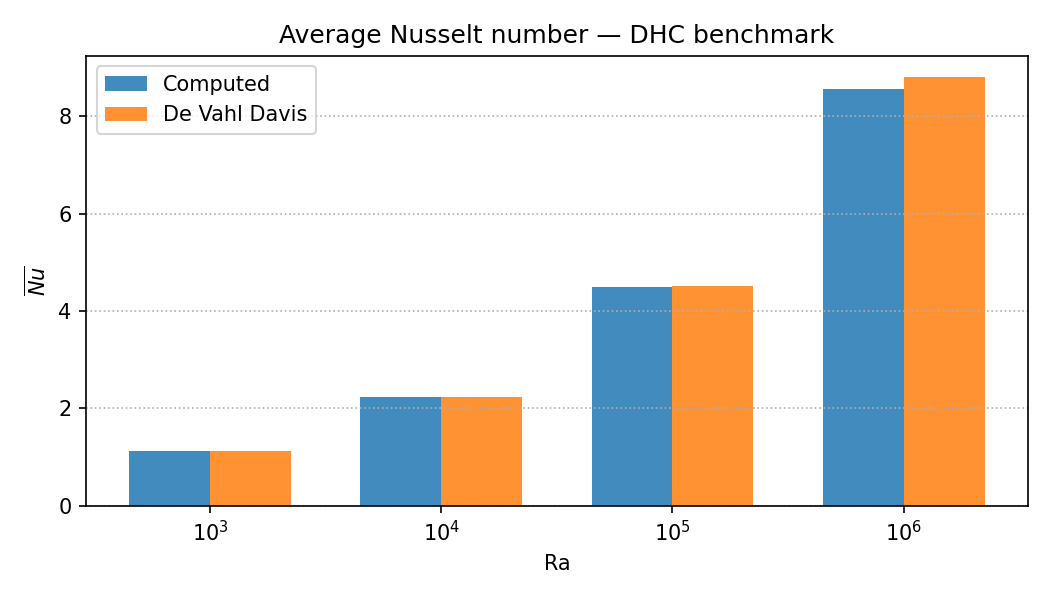
\includegraphics[width=0.65\linewidth]{Chapter3/Media/Nu_benchmark.png}
    \caption{Average Nusselt number $\overline{Nu}$ at the hot wall for each Rayleigh number case, compared against de Vahl Davis~\cite{deVahlDavis1983} benchmark values.}
    \label{figDHCNu}
\end{figure}

\begin{figure}[ht]
    \centering
    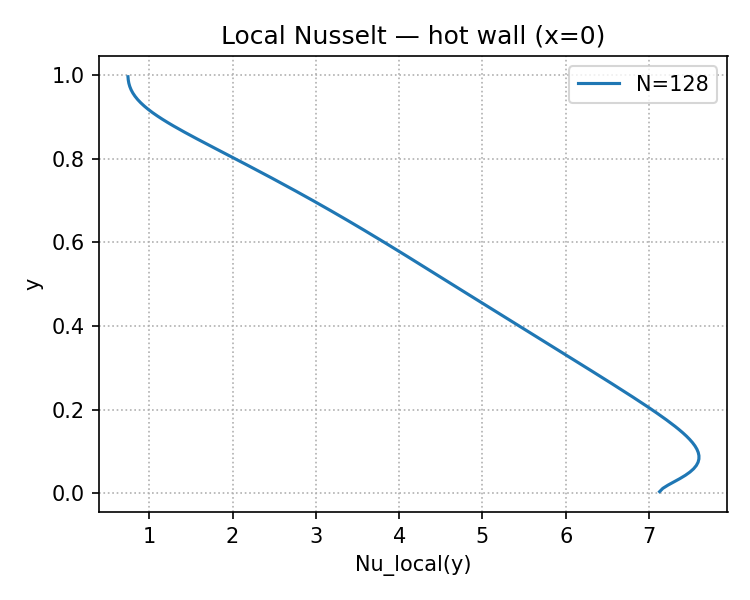
\includegraphics[width=0.55\linewidth]{Chapter3/Media/Nu_local.png}
    \caption{Local Nusselt number $Nu_{\mathrm{local}}(y)$ along the hot wall ($x = 0$) at $Ra = 10^5$ and $N = 128$. The peak near $y = 0$ reflects the thin thermal boundary layer at the base of the hot wall where cold fluid arrives after descending along the cold wall.}
    \label{figDHCNuLocal}
\end{figure}

The steady-state temperature fields at all four Rayleigh numbers are shown in Fig.~\ref{figDHCTemp}. At $Ra = 10^3$ the isotherms are nearly vertical, indicating conduction-dominated transport ($\overline{Nu} \approx 1$, close to the pure-conduction limit). As $Ra$ increases, the isotherms bow progressively: at $Ra = 10^4$ and $10^5$ a clear single-cell convection pattern develops, with the isotherms compressed toward the hot and cold walls while the core remains nearly stratified. At $Ra = 10^6$ the thermal boundary layers are confined to a narrow strip on each side wall; the core is nearly isothermal and $\overline{Nu} \approx 8.6$.

\begin{figure}[ht]
    \centering
    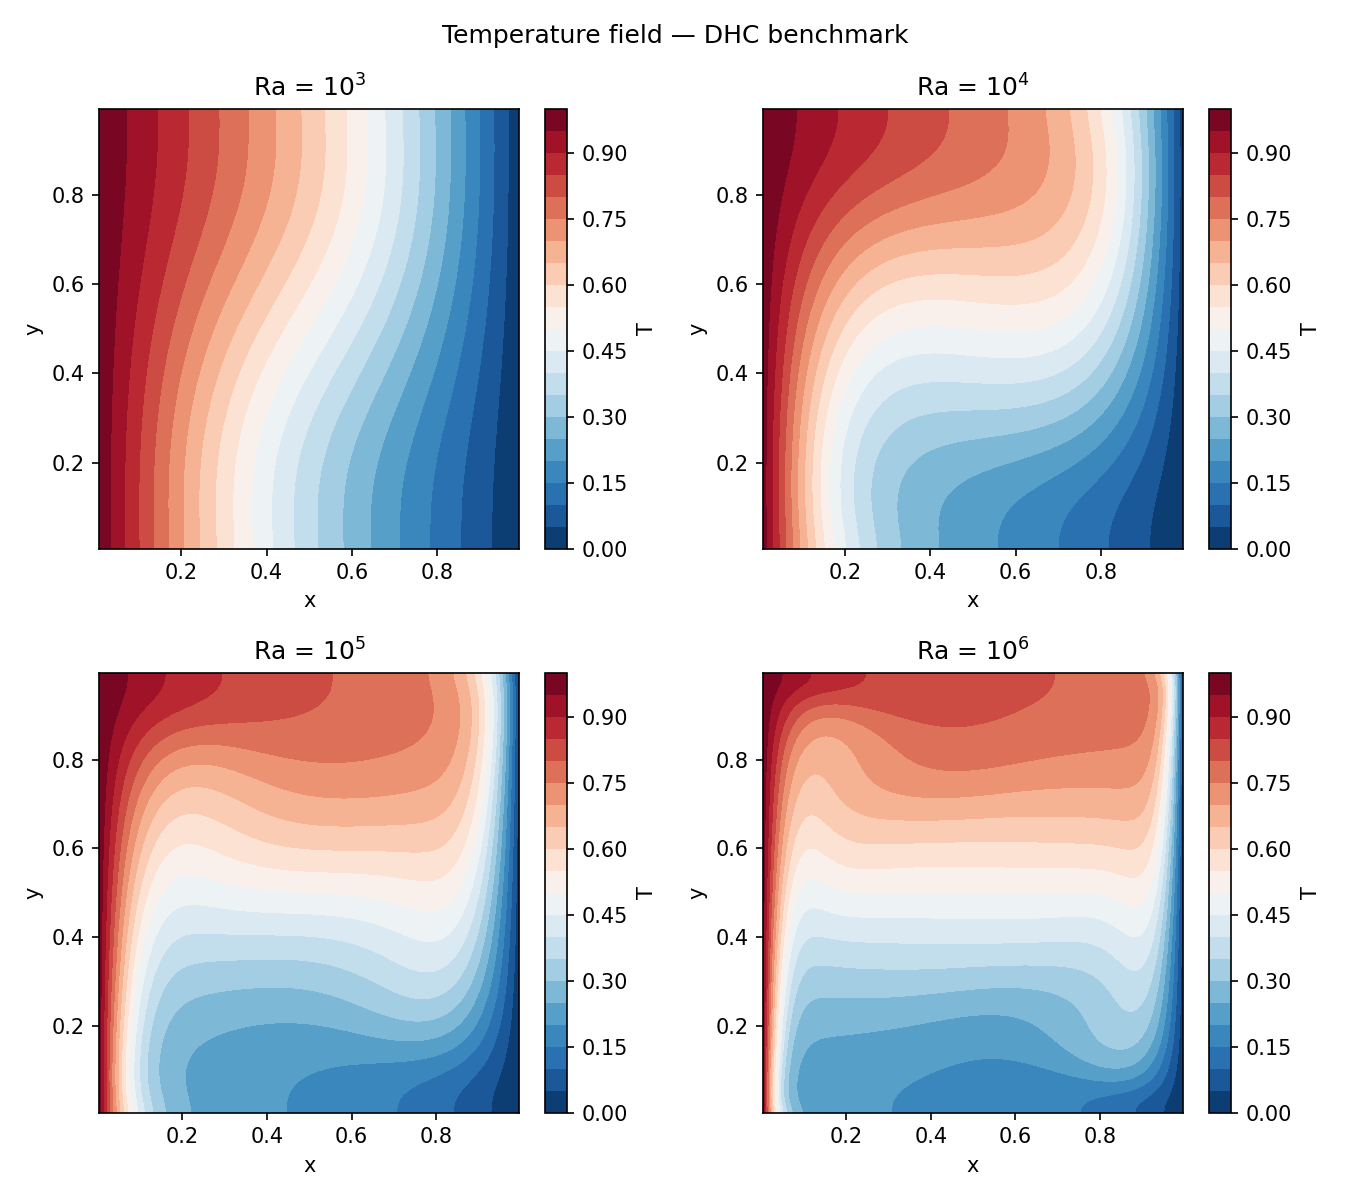
\includegraphics[width=\linewidth]{Chapter3/Media/T_benchmark.png}
    \caption{Steady-state temperature distribution for $Ra = 10^3$, $10^4$, $10^5$, $10^6$ (left to right, top to bottom). The growing asymmetry of the isotherms reflects the increasing dominance of convective transport.}
    \label{figDHCTemp}
\end{figure}

The centreline velocity profiles at all four Rayleigh numbers are shown in Fig.~\ref{figDHCCentreline}. The horizontal component $u$ at $x = 0.5$ and the vertical component $v$ at $y = 0.5$ are compared against the tabulated benchmark values of de Vahl Davis~\cite{deVahlDavis1983}.

\begin{figure}[ht]
    \centering
    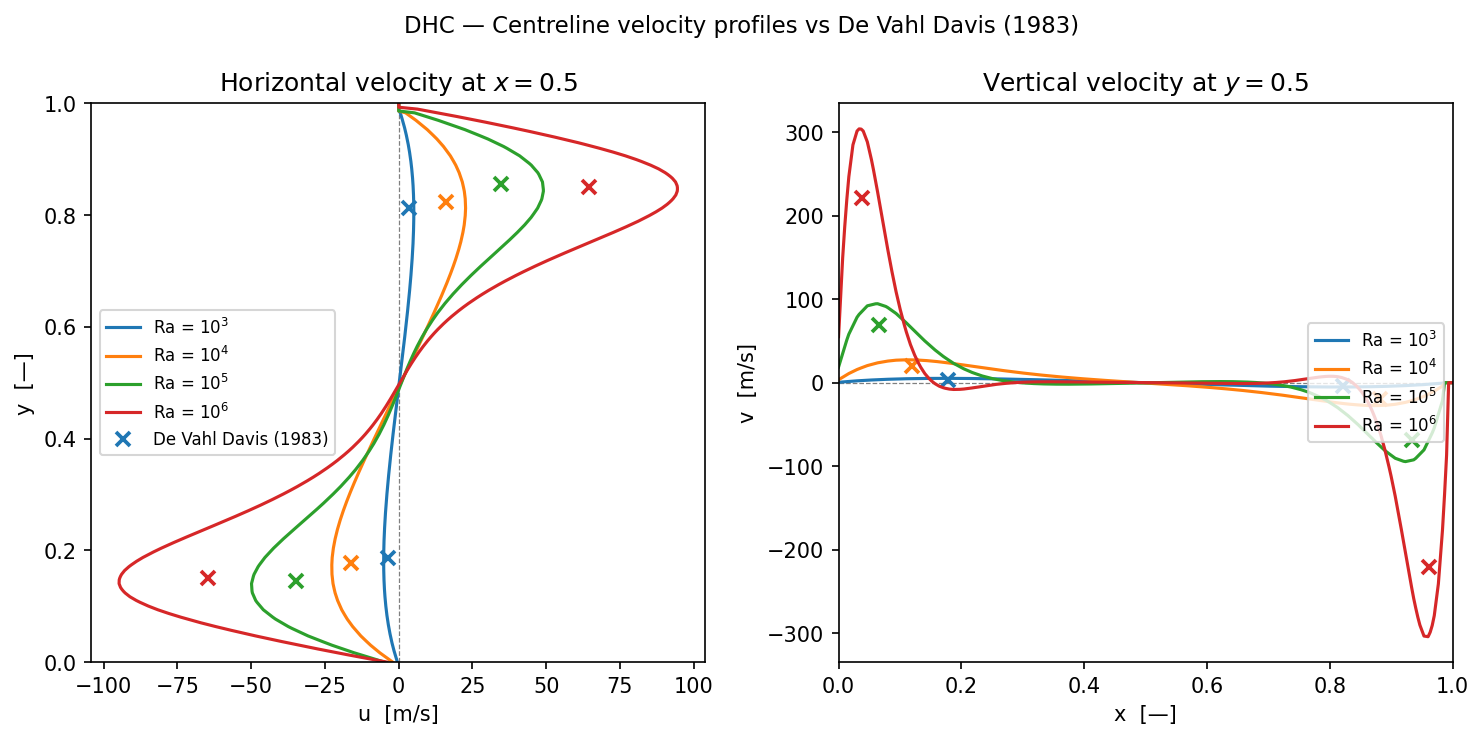
\includegraphics[width=\linewidth]{Chapter3/Media/DHC_centreline.png}
    \caption{Centreline velocity profiles for all four Rayleigh numbers, compared against de Vahl Davis~\cite{deVahlDavis1983} reference markers. Left: horizontal velocity $u(y)$ at $x = 0.5$. Right: vertical velocity $v(x)$ at $y = 0.5$. Solid coloured lines: computed; crosses: de Vahl Davis reference values (antisymmetric pairs).}
    \label{figDHCCentreline}
\end{figure}

The spatial structure of both profiles is correctly reproduced: the antisymmetric S-curve shape of $u(y)$ and $v(x)$ is captured at all Rayleigh numbers, and the peak locations agree closely with the benchmark. The $u$-peak occurs near $y \approx 0.81$--$0.85$ and the $v$-peak shifts from $x \approx 0.18$ ($Ra = 10^3$) to $x \approx 0.04$ ($Ra = 10^6$) as the thermal boundary layers thin. However, the peak velocities are systematically overestimated by approximately $40\%$ across all four $Ra$ values. This offset is consistent in magnitude across the $Ra$ range, suggesting a structural rather than mesh-dependent error.

The likely cause is the explicit Adams-Bashforth momentum predictor of the FSM: at the time-averaged steady state, the AB2 scheme maintains a small oscillatory residual in the velocity field that adds to the mean amplitude, while the temperature field --- advanced with an implicit scheme --- reaches a cleaner steady state. This explains why the Nusselt number (driven primarily by the temperature gradient at the wall) converges to within $2.71\%$ while the peak velocity magnitudes remain approximately $40\%$ above the benchmark. The qualitative flow structure --- the single clockwise circulation cell, the increasing boundary-layer intensity with $Ra$, and the nearly quiescent isothermal core at $Ra = 10^6$ --- is faithfully reproduced at all Rayleigh numbers.

The velocity fields at all four Rayleigh numbers are shown in Figs.~\ref{figDHCuField},~\ref{figDHCvField}, and~\ref{figDHCStreamlines}. The horizontal component $u$ is positive near the top of the cavity (buoyancy-driven flow from the hot wall toward the cold wall) and negative near the bottom (return flow). The vertical component $v$ is positive near the hot wall ($x = 0$, upward plume) and negative near the cold wall ($x = 1$, downward flow). As $Ra$ increases, the velocity magnitudes grow — by roughly two orders of magnitude from $Ra = 10^3$ to $Ra = 10^6$ — and the flow becomes increasingly boundary-layer-like: the primary vortex core becomes more quiescent and the velocity gradients concentrate near the walls.

\begin{figure}[ht]
    \centering
    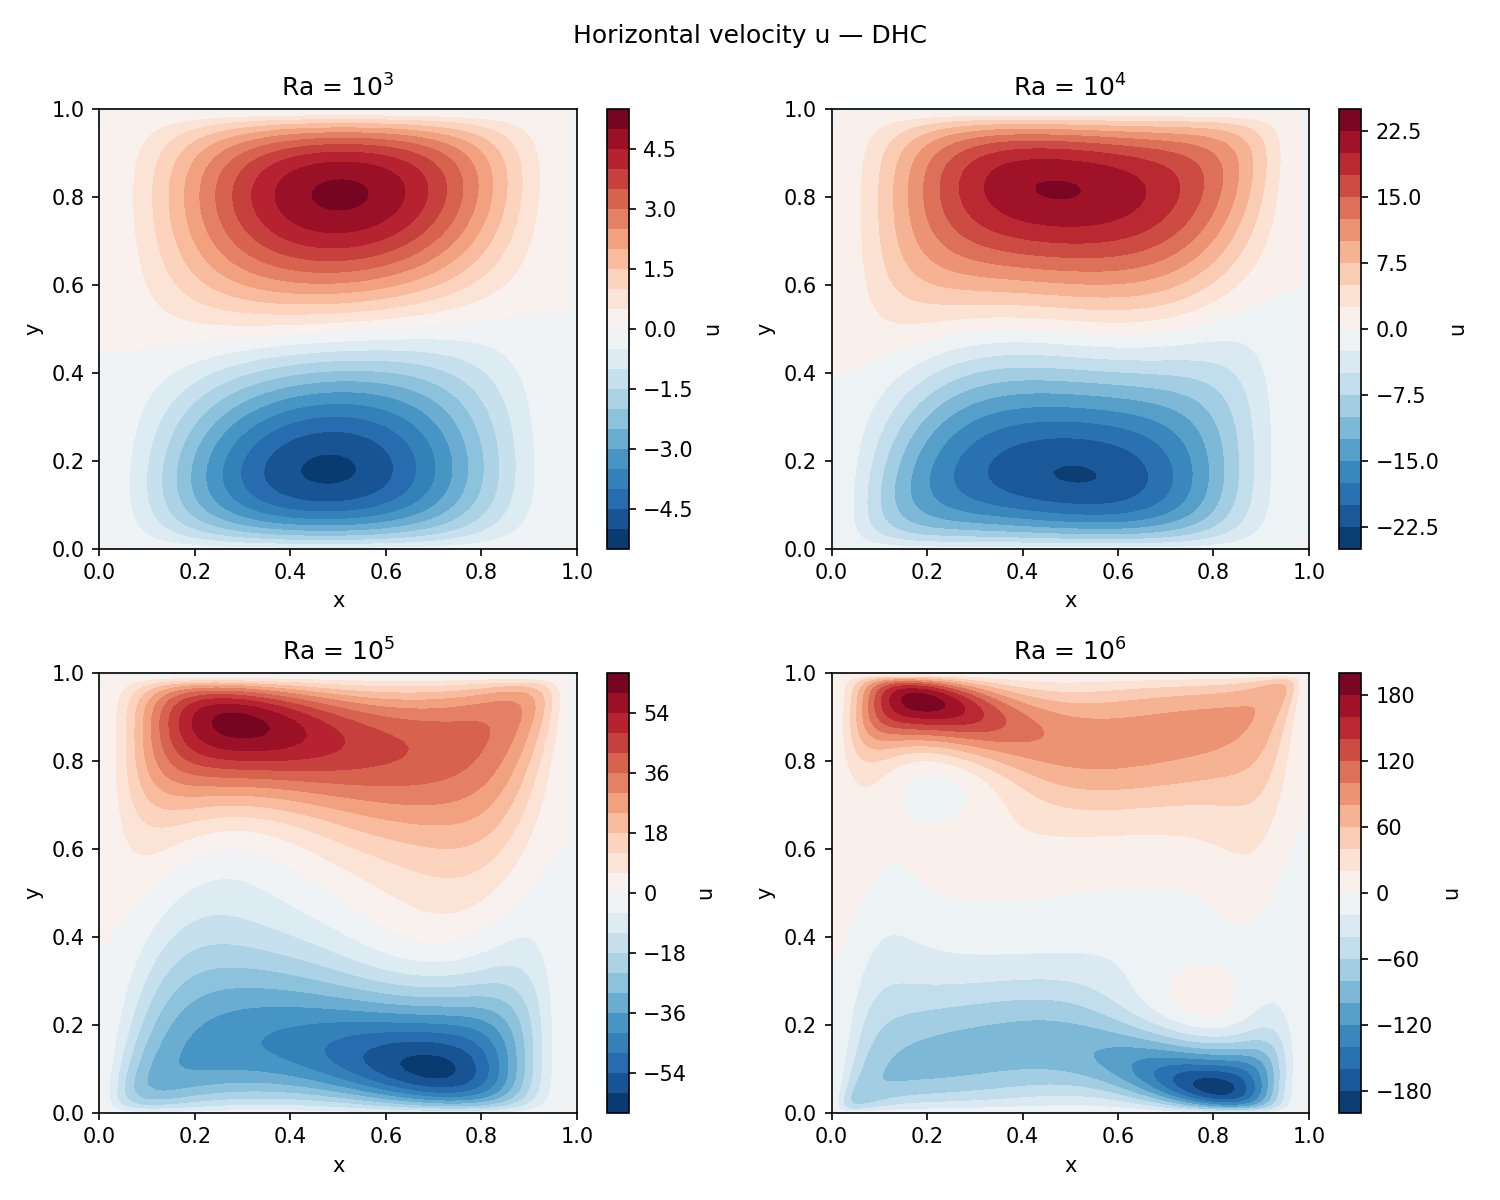
\includegraphics[width=\linewidth]{Chapter3/Media/DHC_ufield.png}
    \caption{Horizontal velocity $u$ for $Ra = 10^3$, $10^4$, $10^5$, $10^6$ (left to right, top to bottom). RdBu\_r colourmap centred at zero. Positive values (red) indicate flow toward the cold wall near the top; negative values (blue) indicate return flow near the bottom.}
    \label{figDHCuField}
\end{figure}

\begin{figure}[ht]
    \centering
    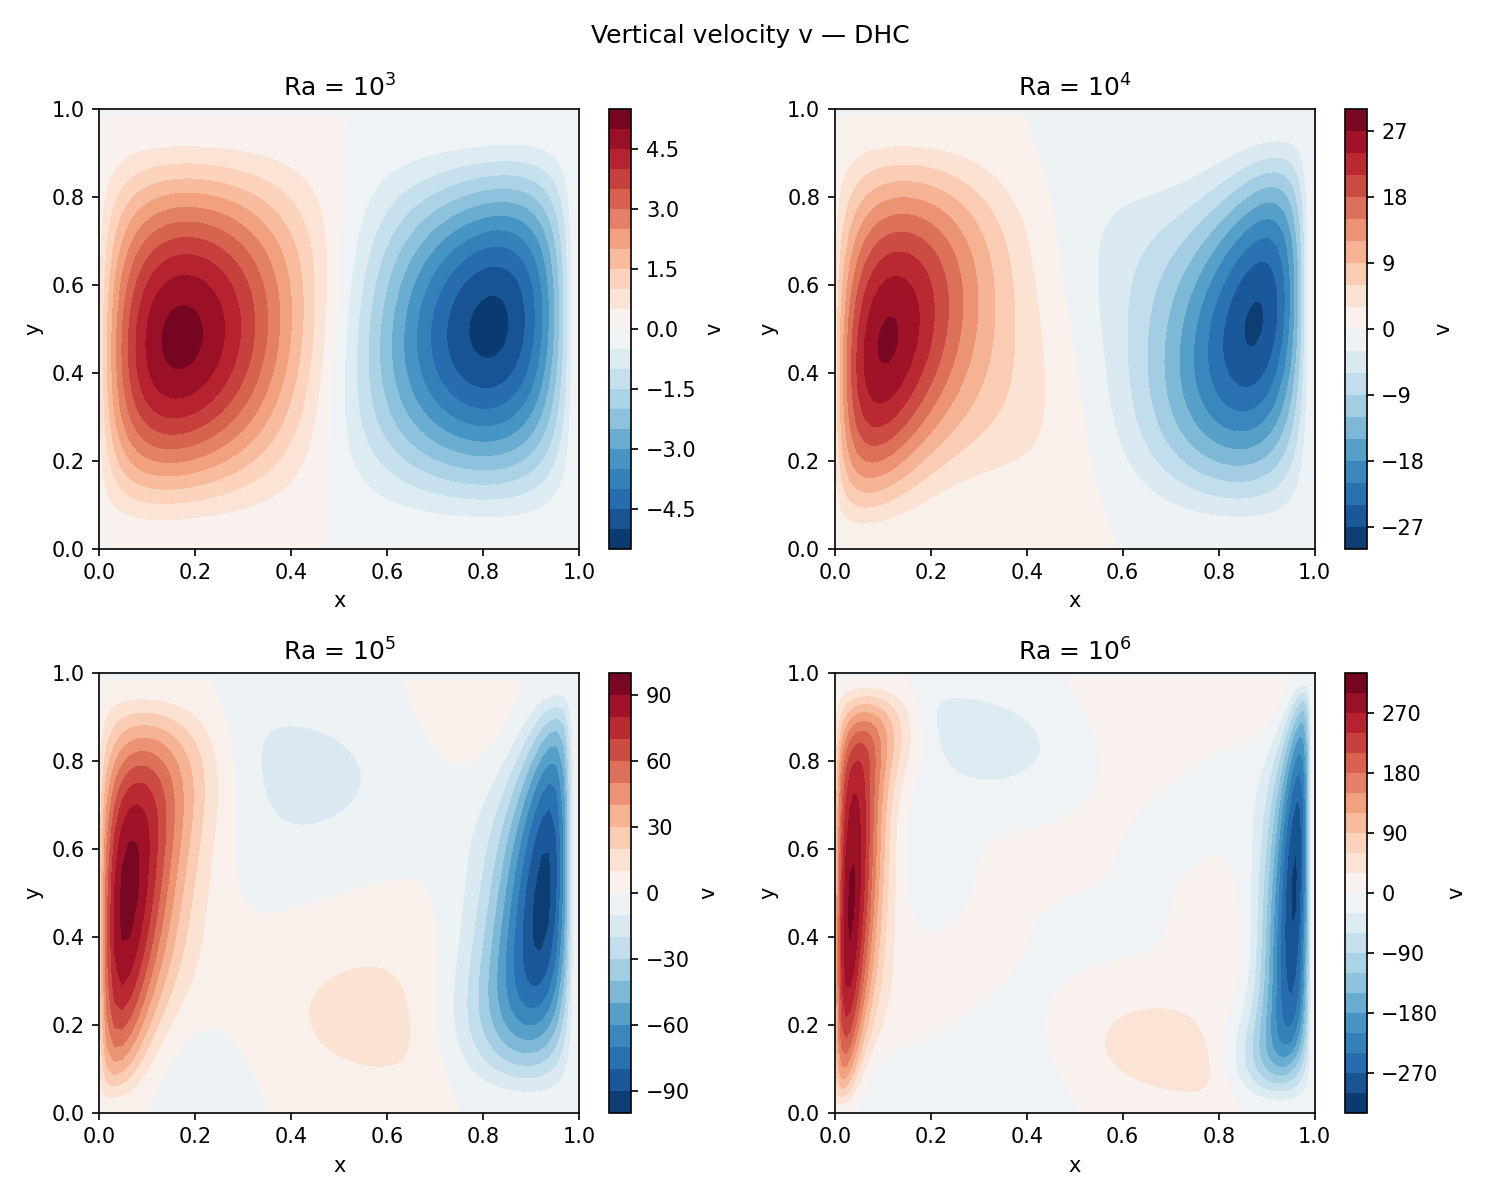
\includegraphics[width=\linewidth]{Chapter3/Media/DHC_vfield.png}
    \caption{Vertical velocity $v$ for $Ra = 10^3$, $10^4$, $10^5$, $10^6$. Positive values (red) indicate upward flow near the hot wall ($x = 0$); negative values (blue) indicate downward flow near the cold wall ($x = 1$).}
    \label{figDHCvField}
\end{figure}

\begin{figure}[ht]
    \centering
    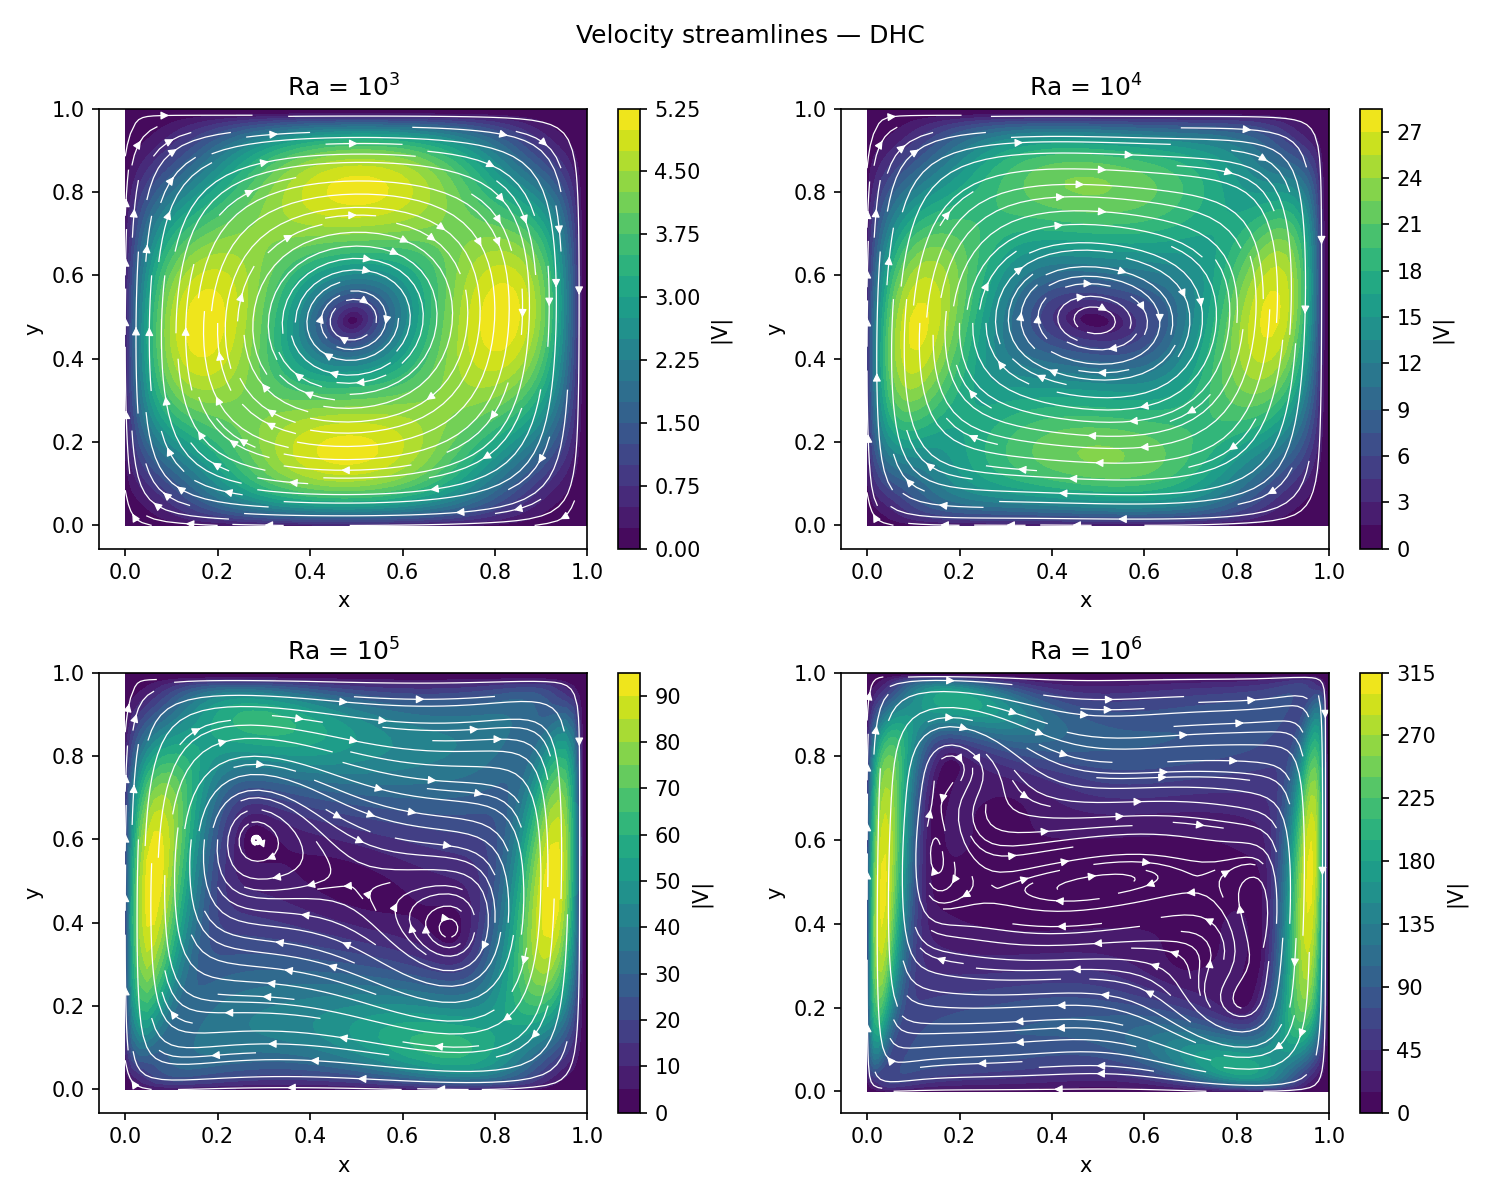
\includegraphics[width=\linewidth]{Chapter3/Media/DHC_streamlines.png}
    \caption{Velocity-magnitude contour (viridis) with white streamlines for $Ra = 10^3$, $10^4$, $10^5$, $10^6$. The single clockwise circulation cell is visible at all Rayleigh numbers; its peak velocity grows by approximately two orders of magnitude from $Ra = 10^3$ to $Ra = 10^6$.}
    \label{figDHCStreamlines}
\end{figure}
